\documentclass[a4paper,twoside,master.tex]{subfiles}
\begin{document}
\lecture{29}{Wednesday, October 30, 2019}{Potential Scattering}

First, some review of the exam:
\begin{equation}
    \ket{\psi_0} = \frac{1}{\sqrt{3}} (\ket{A} + \ket{B} + \ket{C})
\end{equation}
and
\begin{equation}
    \ket{F} = \frac{1}{\sqrt{3}} (\ket{A} + \ket{B} - \ket{C})
\end{equation}
\begin{equation}
    Y^1 = [\psi_0]\odot[A]\odot[F]
\end{equation}
so
\begin{equation}
    \ket{\psi^1} = [F][A] \ket{\psi_0} = [F] \frac{1}{\sqrt{3}} \ket{A} = \frac{1}{3} \ket{F}
\end{equation}
Next,
\begin{equation}
    Y^2 = [\psi_0]\odot[A]\odot(I-[F])
\end{equation}
so
\begin{equation}
    \ket{Y^2} = (I-[F])[A] \ket{\psi_0} = (I-[F]) \frac{1}{\sqrt{3}} \ket{A} 
\end{equation}
Instead of writing out $ I - [F] $, we can just distribute:
\begin{equation}
    \ket{Y^2} = \frac{1}{\sqrt{3}} \ket{A} - \frac{1}{3} \ket{F}
\end{equation}

Let's look at one of the probability questions now:
\begin{equation}
    \Pr([A]_1\mid[\psi_0][F_1]) = \frac{\Pr(\psi_0,A_1,F_2)}{\Pr(\psi_0,F_1)} = \frac{\Pr(Y^1) = \frac{1}{9}}{\Pr(Y^1)+\Pr(Y^3) = \frac{1}{9} + 0} = 1
\end{equation}

Now back to potential scattering:

\subsection{Square Well Scattering}
\label{sub:square_well_scattering}

\begin{equation}
    V(x) = \begin{cases} -V_0 & \abs{x} > a/2 \\ 0 & \abs{x} < a/2 \end{cases}
\end{equation}
We know solutions are exponential, proportional to $ e^{\pm\imath kx} $ with $ k = \sqrt{E} $ outside the well and $ e^{\pm\imath k'x} $ with $ k' = \sqrt{V_0 + E} > k $ inside the well.

\begin{equation}
    \phi = \begin{cases}
        A e^{\imath k x} + B e^{-\imath k x}& x < -a/2\\
        C e^{\imath k'x} + D e^{-\imath k'x}& -a/2 < x < a/2\\
        F e^{\imath k x} + G e^{-\imath k x}& a/2 < x\\
    \end{cases}
\end{equation}
Boundary conditions at $ -a/2 $ give us
\begin{equation}
    A e^{-\imath ka/2} + B e^{\imath ka/2} = C e^{-\imath k'a/2} + D e^{\imath k'a/2}
\end{equation}
and
\begin{equation}
    \underbrace{kA e^{-\imath ka/2} - kB e^{\imath ka/2}}_{P\begin{pmatrix}A\\B\end{pmatrix}} = \underbrace{k'C e^{-\imath k'a/2} - k'D e^{\imath k'a/2}}_{Q\begin{pmatrix}C\\D\end{pmatrix}}
\end{equation}
so
\begin{equation}
    \begin{pmatrix}A\\B\end{pmatrix} = P^{-1}Q\begin{pmatrix}C\\D\end{pmatrix}
\end{equation}
where $ P^{-1}Q = R $.

By time reversal symmetry (taking the complex conjugate of $ \varphi $ and noting that the Schr\"odinger equation is invariant under this operation), we can conclude that
\begin{equation}
    \begin{pmatrix}A^*\\B^*\end{pmatrix} = R\begin{pmatrix}C^*\\D^*\end{pmatrix}
\end{equation}
so $ R^*_{11} = R_{22} $ and $ R^*_{12} = R_{21} $
\begin{equation}
    R = \sqrt{\frac{k'}{k}} \begin{pmatrix} \alpha & \beta\\\beta^* & \alpha^*\end{pmatrix}
\end{equation}
The incident current is
\begin{equation}
    J_{\text{inc}} = k(\abs{A}^2 - \abs{B}^2) = J_{\text{transf}} = k'(\abs{C}^2 - \abs{D}^2)
\end{equation}
therefore,
\begin{equation}
    \abs{\alpha}^2 - \abs{\beta}^2 = 1
\end{equation}
or
\begin{equation}
    \det{\begin{pmatrix} \alpha & \beta\\\beta^* & \alpha^*\end{pmatrix}} = 1
\end{equation}

Applying the same method of time-reversal and current conservation to the other boundary. We can reuse $ R $ evaluated at any other point in space (called $ \tilde{R} $). Therefore
\begin{equation}
    \begin{bmatrix}
        A\\B
    \end{bmatrix}
    =\underbrace{R\tilde{R}}_{M} 
    \begin{bmatrix}
        F\\G
    \end{bmatrix}
\end{equation}
\begin{equation}
    M=
    \begin{bmatrix}
        \gamma & \delta \\ \delta^* & \gamma^*
    \end{bmatrix}
\end{equation}
\begin{equation}
    \abs{\gamma}^2 - \abs{\delta}^2 = 1
\end{equation}
so
\begin{equation}
    \gamma = \alpha^2 - \beta^2 = e^{\imath ka} \left[ \cos(k'a) -\imath \frac{k^2 + k'^2}{2kk'} \sin(k'a) \right]
\end{equation}
is the reflection coefficient.

For transmission, set $ A=1 $, and we want $ G=0 $. Our equation now becomes
\begin{equation}
    \begin{bmatrix}
        1\\B
    \end{bmatrix}
    = M 
    \begin{bmatrix}
        F\\0
    \end{bmatrix}
\end{equation}
so
\begin{equation}
    F = \frac{1}{M_{11}}
\end{equation}
and
\begin{equation}
    T = \abs{F}^2 = \frac{1}{\abs{\gamma}^2} = \frac{1}{1 + \frac{(k^2 - k'^2 )^2}{2 k^2 k'^2} \sin^2(k'a)}
\end{equation}
Recall that $ k' = \sqrt{V_0 + k^2} $, so plotting the coefficients as a function of $ k $, we see the following result:
\begin{figure}[h]
    \centering
    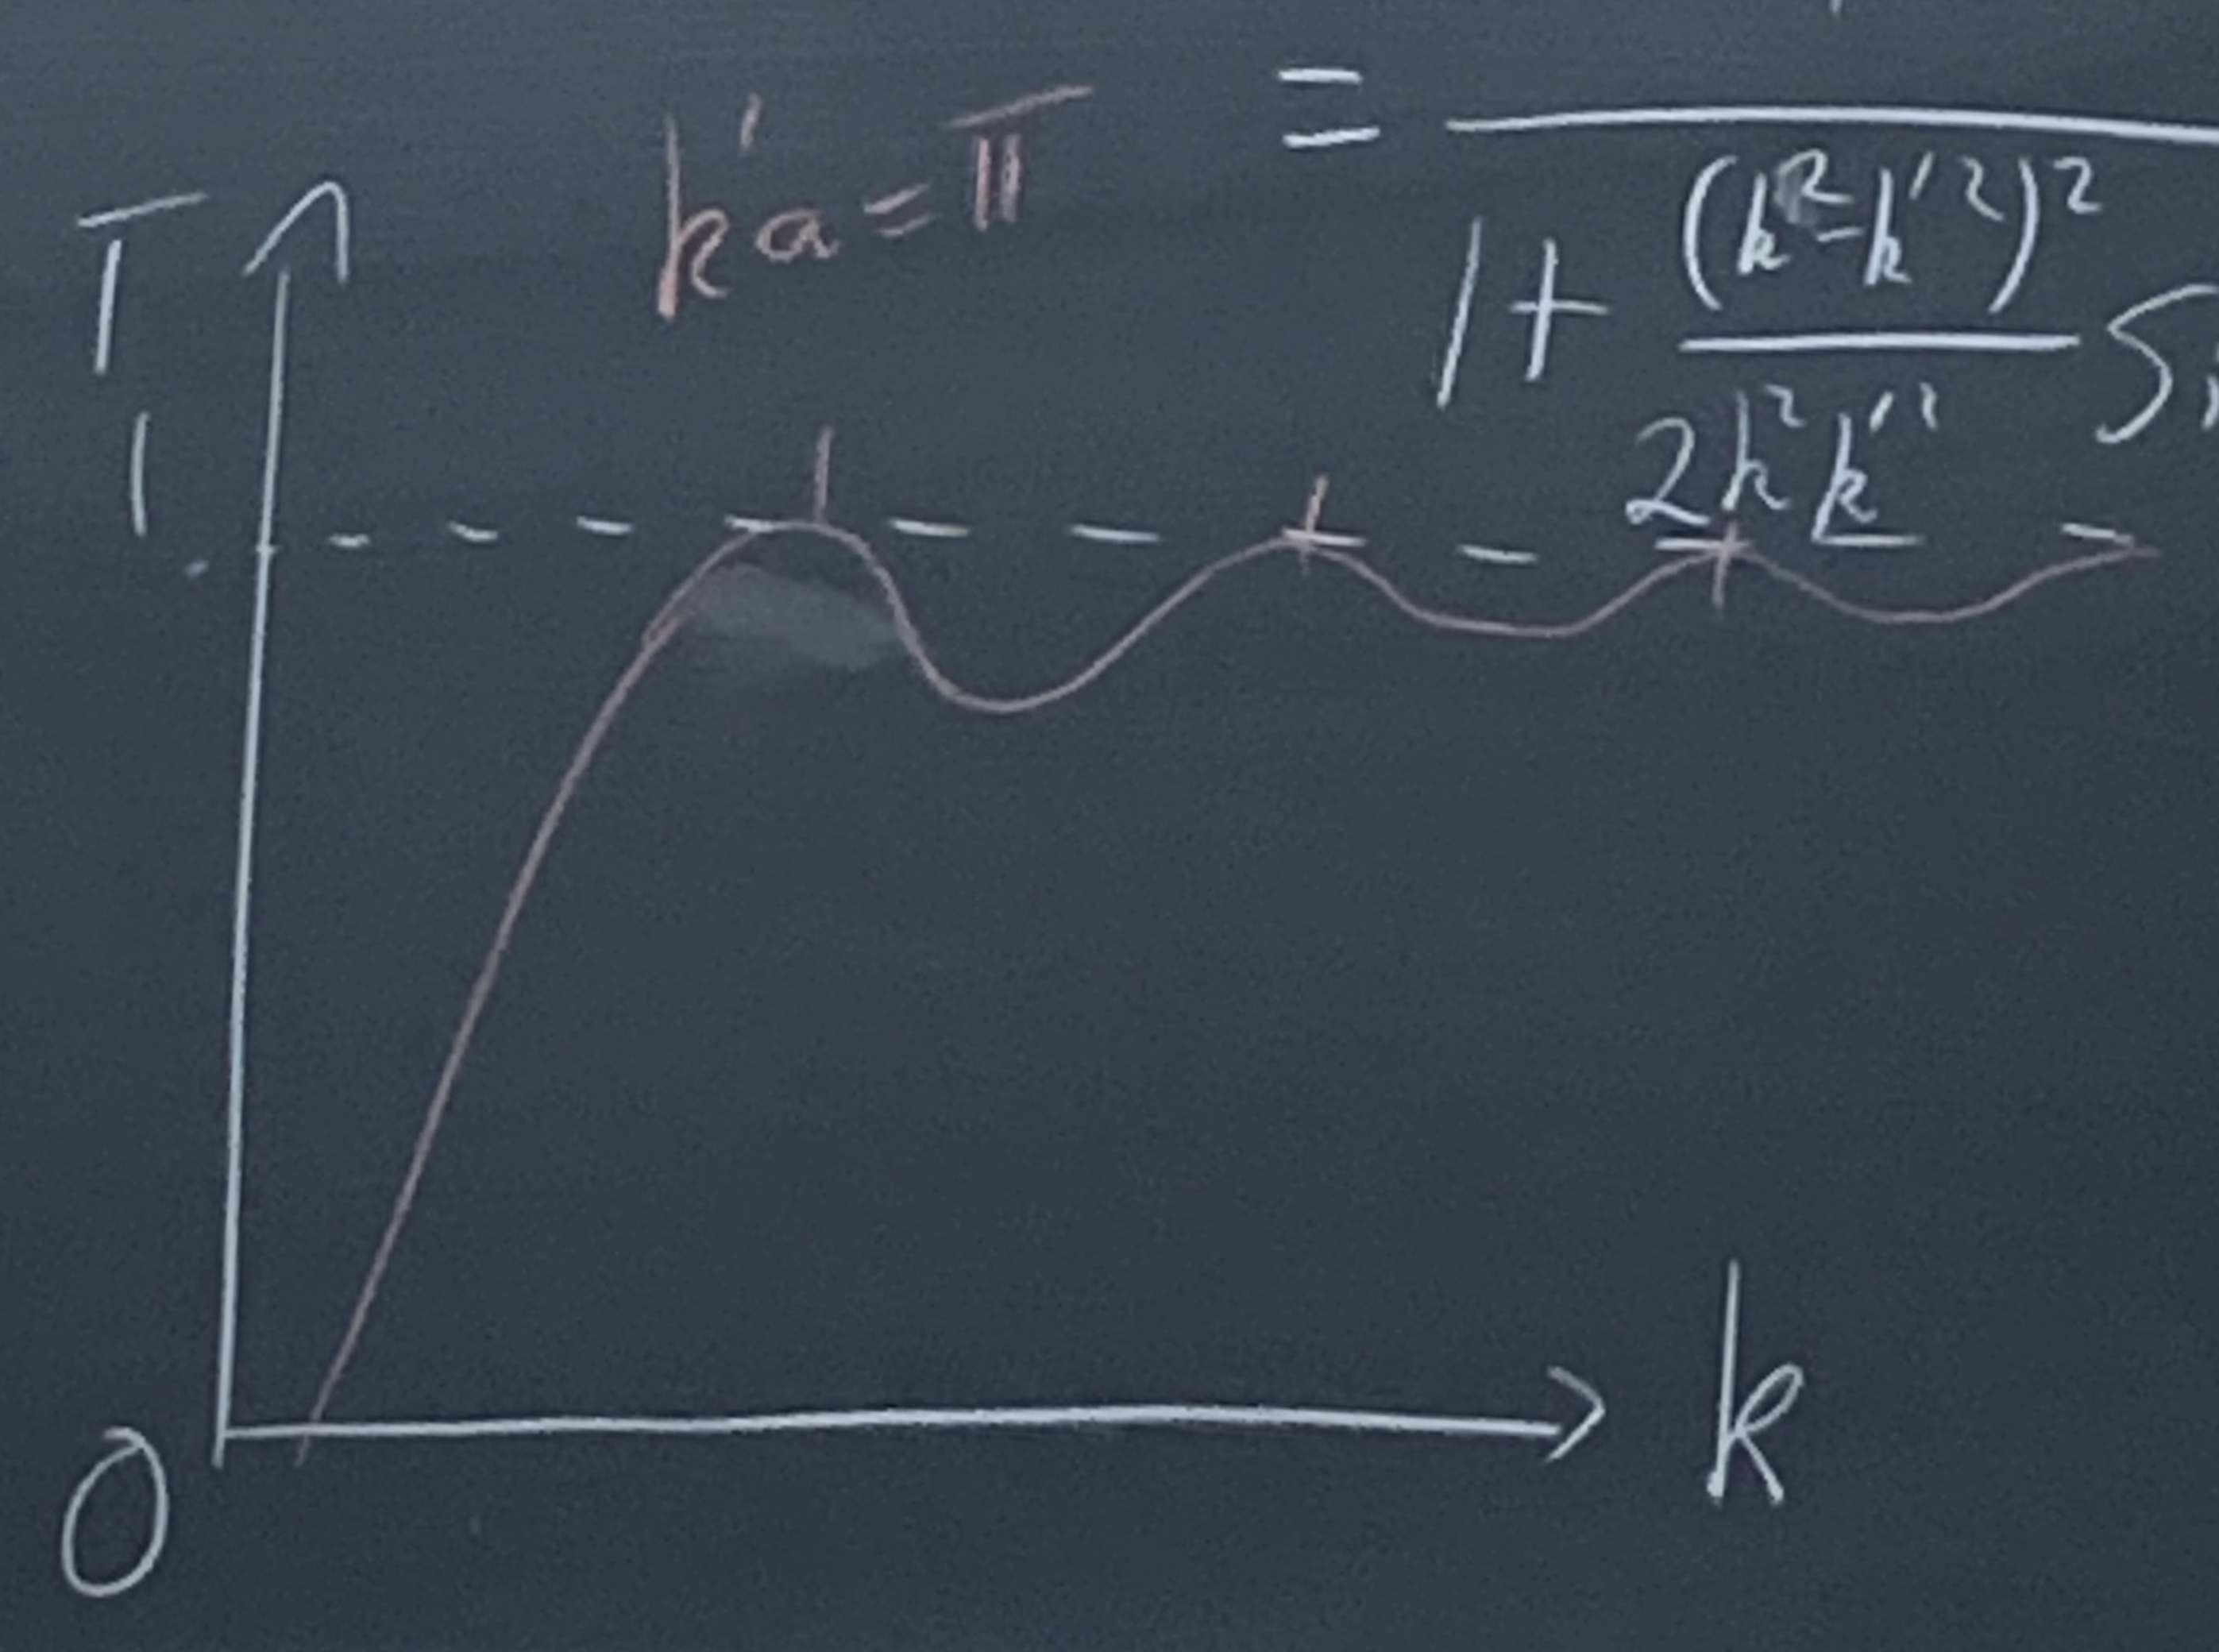
\includegraphics[width=\textwidth/2]{figures/lec_29_k_vs_T.jpg}
    \caption{Graph of $ k $ vs $ T $}
    \label{fig:k_vs_T_square_well}
\end{figure}


\end{document}
